\section{Discussion of backgrounds}
\label{sec:bkgtypes}

As shown in Section~\ref{sec:yields}, the SM background to this study is dominated 
by \ttbar events. The contribution from single-top, diboson production ($WZ, ZZ$), 
are small. The diboson backgrounds will come almost entirely from Monte Carlo. 
The Monte Carlo acceptances for these processes will be corrected for differences in 
data and Monte Carlo lepton identification and trigger efficiencies, as determined from 
the tag-and-probe method.

We study the same signed dileptons for the dominant \ttbar background based on their origins.
Typically, dileptons are produced via top decays, $t \rightarrow W b$; where 
$W \rightarrow \ell \nu $, based on the truth matched to their ``parents'' we classify them 
into the following types.

\begin{itemize}
\item Type-I: Both leptons originate from real $W$ bosons, one with mis-reconstructed charge.
\item Type-II a): One of the lepton is from real $W$ and the other originate from heavy flavor sources ($b, c$).
\item Type-II b): One of the lepton is from $W$ and the other is a fake lepton.
\item Type-III: Both leptons are not from $W$ and are fakes.
\end{itemize} 

\begin{figure}[htb]
\begin{center}
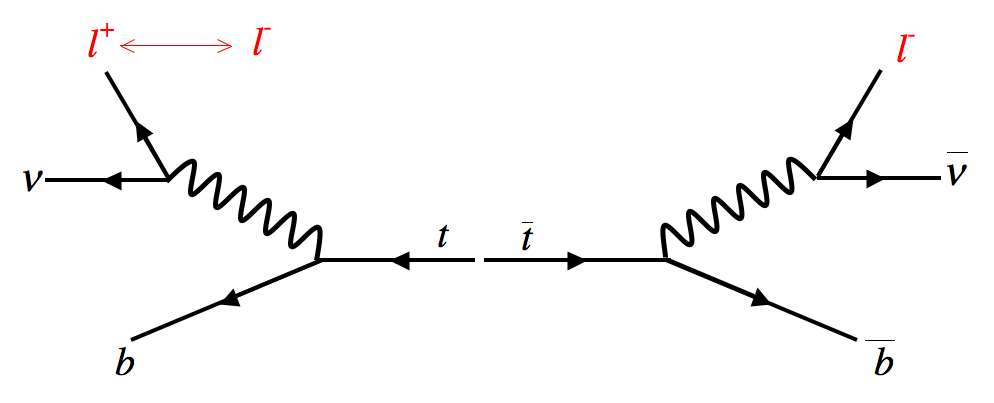
\includegraphics[width=0.32\linewidth, height=0.2\linewidth]{figs/feyntypeI.png}
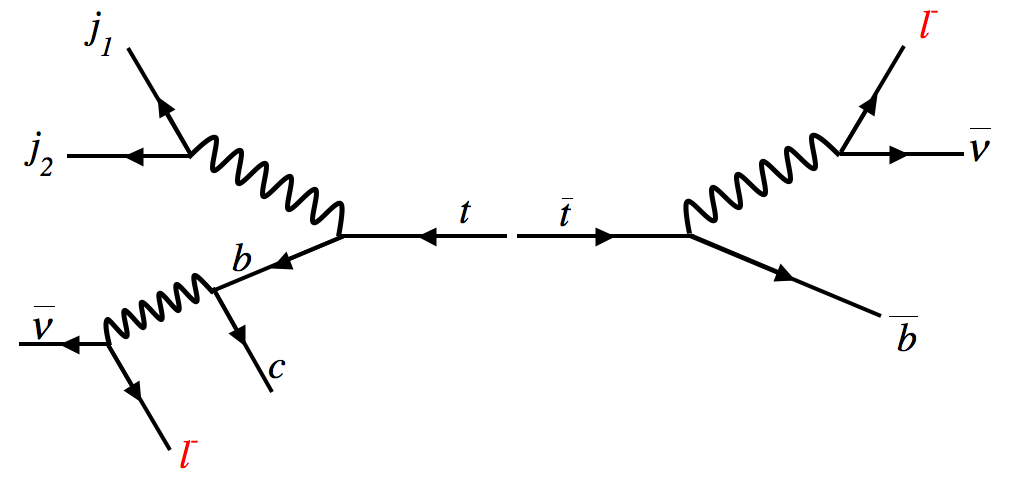
\includegraphics[width=0.32\linewidth, height=0.2\linewidth]{figs/feyntypeIIa.png}
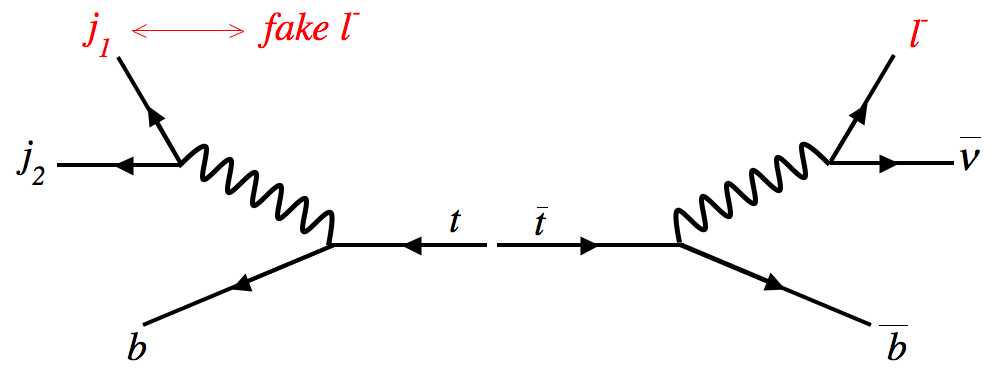
\includegraphics[width=0.32\linewidth, height=0.2\linewidth]{figs/feyntypeIIb.png}
\caption{ Classification of same sign dileptons from \ttbar decays. a) Lepton from $W$ with mis-reconstructed charge; 
b) One of the lepton is from $W$, the other originating from heavy flavor sources; c) One of the lepton is from $W$,
and the other is a fake lepton. \label{fig:fakeOrigin}}
\end{center}
\end{figure}

Figure~\ref{fig:fakeOrigin} illustrates various contribution of background types in \ttbar decays. The MC 
expectations to these contributions are given in Table~\ref{tab:fakeOrigin}.

\begin{table}[hbt]
\begin{center}
\begin{tabular}{|l|c|c|c|c|c|c|}\hline
Same Sign leptons & Total & 	 Type-I &  Type-II & Type-II a) & Type-II b) & Type-III \\ \hline
$ee$ &	0.44 &	0.09 &	0.35 &	0.17 &	0.17 &	0.00 \\
$\mu \mu$ & 	0.13 &	0.00 &	0.13 &	0.13 &	0.00 &	0.00 \\
$e\mu$ &	0.39 &	0.13 &	0.26 &	0.26 &	0.00 &	0.00 \\
Total &	0.96 &	0.22 &	0.74 &	0.57 &	0.17 &	0.00 \\
\hline
\end{tabular}
\caption{ Expected number of \ttbar events for various types in 100 pb$^{-1}$ of integrated luminosity.\label{tab:fakeOrigin}}
\end{center}
\end{table}

It is interesting to note the following:
\begin{itemize}
\item About $\approx 23 \%$ of the contribution is from Type-I (Charge mis-identification).
\item Almost all of the charge mis-identification is from electrons, in $ee$ and $e\mu$ channel.
\item The bulk of the \ttbar contribution in our event selection is from Type-II. The dominant among them 
is due to heavy flavor sources ($\approx 60 \%$)
\item No events with both leptons being fake (Type-III) are found.
\end{itemize} 

In the following sections, we will briefly describe two different data driven approaches to 
estimate the above mentioned contributions. Type-I, contribution will be estimated using ``Charge-flip rate'', 
where as Type-II part will be estimated used Lepton Fake rate method~\cite{fakelep}.



